\begin{figure}[H]	
  \centering
    \resizebox{\linewidth}{!}{\tikzset{font=\Huge}\documentclass{standalone}
\usepackage{tikz}
\usepackage{aeguill}
\begin{document}
% generated by Plantuml 1.2018.12      
\definecolor{plantucolor0000}{RGB}{254,254,206}
\definecolor{plantucolor0001}{RGB}{168,0,54}
\definecolor{plantucolor0002}{RGB}{169,220,223}
\definecolor{plantucolor0003}{RGB}{0,0,0}
\definecolor{plantucolor0004}{RGB}{173,209,178}
\definecolor{plantucolor0005}{RGB}{255,255,255}
\begin{tikzpicture}[yscale=-1
,pstyle0/.style={color=plantucolor0001,fill=plantucolor0000,line width=1.5pt}
,pstyle2/.style={color=plantucolor0001,line width=1.5pt}
,pstyle3/.style={color=plantucolor0001,fill=plantucolor0004,line width=1.0pt}
,pstyle4/.style={color=plantucolor0001,line width=1.0pt}
]
\draw[pstyle0] (6pt,8pt) rectangle (118.2286pt,94.4141pt);
\draw[color=plantucolor0001,fill=plantucolor0002,line width=1.0pt] (21pt,24pt) ellipse (11pt and 11pt);
\node at (21pt,24pt)[]{\textbf{\Large A}};
\node at (35pt,17.0156pt)[below right,color=black]{\textit{Component}};
\draw[pstyle2] (7pt,40pt) -- (117.2286pt,40pt);
\draw[pstyle2] (7pt,48pt) -- (117.2286pt,48pt);
\node at (12pt,52pt)[below right,color=black]{\textit{method1()}};
\node at (12pt,64.8047pt)[below right,color=black]{\textit{method2()}};
\node at (12pt,77.6094pt)[below right,color=black]{\textit{method3()}};
\draw[pstyle0] (350pt,154pt) rectangle (527.9748pt,240.4141pt);
\draw[pstyle3] (365pt,170pt) ellipse (11pt and 11pt);
\node at (365pt,170pt)[]{\textbf{\Large C}};
\node at (379pt,163.0156pt)[below right,color=black]{ConcreteComponent};
\draw[pstyle2] (351pt,186pt) -- (526.9748pt,186pt);
\draw[pstyle2] (351pt,194pt) -- (526.9748pt,194pt);
\node at (356pt,198pt)[below right,color=black]{method1()};
\node at (356pt,210.8047pt)[below right,color=black]{method2()};
\node at (356pt,223.6094pt)[below right,color=black]{method3()};
\draw[pstyle0] (10.5pt,166.5pt) rectangle (113.3393pt,227.3047pt);
\draw[pstyle3] (25.5pt,182.5pt) ellipse (11pt and 11pt);
\node at (25.5pt,182.5pt)[]{\textbf{\Large C}};
\node at (39.5pt,175.5156pt)[below right,color=black]{Decorator};
\draw[pstyle2] (11.5pt,198.5pt) -- (112.3393pt,198.5pt);
\node at (16.5pt,202.5pt)[below right,color=black]{component};
\draw[pstyle2] (11.5pt,219.3047pt) -- (112.3393pt,219.3047pt);
\draw[pstyle0] (148.5pt,154pt) rectangle (315.9769pt,240.4141pt);
\draw[pstyle3] (163.5pt,170pt) ellipse (11pt and 11pt);
\node at (163.5pt,170pt)[]{\textbf{\Large C}};
\node at (177.5pt,163.0156pt)[below right,color=black]{ConcreteDecorator};
\draw[pstyle2] (149.5pt,186pt) -- (314.9769pt,186pt);
\draw[pstyle2] (149.5pt,194pt) -- (314.9769pt,194pt);
\node at (154.5pt,198pt)[below right,color=black]{method1()};
\node at (154.5pt,210.8047pt)[below right,color=black]{method2()};
\node at (154.5pt,223.6094pt)[below right,color=black]{method3()};
\draw[pstyle4] (137.2656pt,79.0956pt) ..controls (191.7443pt,99.5561pt) and (267.0767pt,128.1046pt) .. (333pt,154pt) ..controls (338.5453pt,156.1783pt) and (344.2466pt,158.4365pt) .. (349.9912pt,160.7261pt);
\draw[pstyle4] (134.4625pt,85.5205pt) -- (118.194pt,71.9434pt) -- (139.3785pt,72.412pt) -- (134.4625pt,85.5205pt) -- cycle;
\draw[pstyle4] (49.3526pt,114.2046pt) ..controls (48.972pt,132.2759pt) and (49.6503pt,151.1628pt) .. (51.3873pt,166.3269pt);
\draw[pstyle4] (42.3689pt,113.6812pt) -- (50.2585pt,94.0152pt) -- (56.3549pt,114.3089pt) -- (42.3689pt,113.6812pt) -- cycle;
\draw[pstyle4] (75.178pt,107.2226pt) ..controls (75.7719pt,122.4473pt) and (75.5442pt,138.7013pt) .. (74.4949pt,153.1368pt);
\draw[color=plantucolor0001,fill=white,line width=1.0pt] (73.237pt,166.3269pt) -- (77.7886pt,160.7338pt) -- (74.3763pt,154.3811pt) -- (69.8247pt,159.9742pt) -- (73.237pt,166.3269pt) -- cycle;
\draw[color=plantucolor0001,fill=plantucolor0001,line width=1.0pt] (74.4321pt,94.0152pt) -- (70.9459pt,103.2264pt) -- (74.714pt,99.0072pt) -- (78.9332pt,102.7753pt) -- (74.4321pt,94.0152pt) -- cycle;
\draw[pstyle4] (74.714pt,99.0072pt) -- (75.1652pt,106.9945pt);
\draw[pstyle4] (133.8172pt,197pt) ..controls (138.6871pt,197pt) and (143.5569pt,197pt) .. (148.4267pt,197pt);
\draw[pstyle4] (133.7969pt,203.9999pt) -- (113.7969pt,197pt) -- (133.7968pt,189.9999pt) -- (133.7969pt,203.9999pt) -- cycle;
\end{tikzpicture}
\end{document}
}
\end{figure}
\begin{intentbox}[Intent]
  We have some basic building blocks that share common method declarations
  but may have lots of different functionality.\\
  $\Rightarrow$ attach dynamically additional responsibility to an object by
  passing it to a decorator.
  \begin{figure}[H]
    \centering
    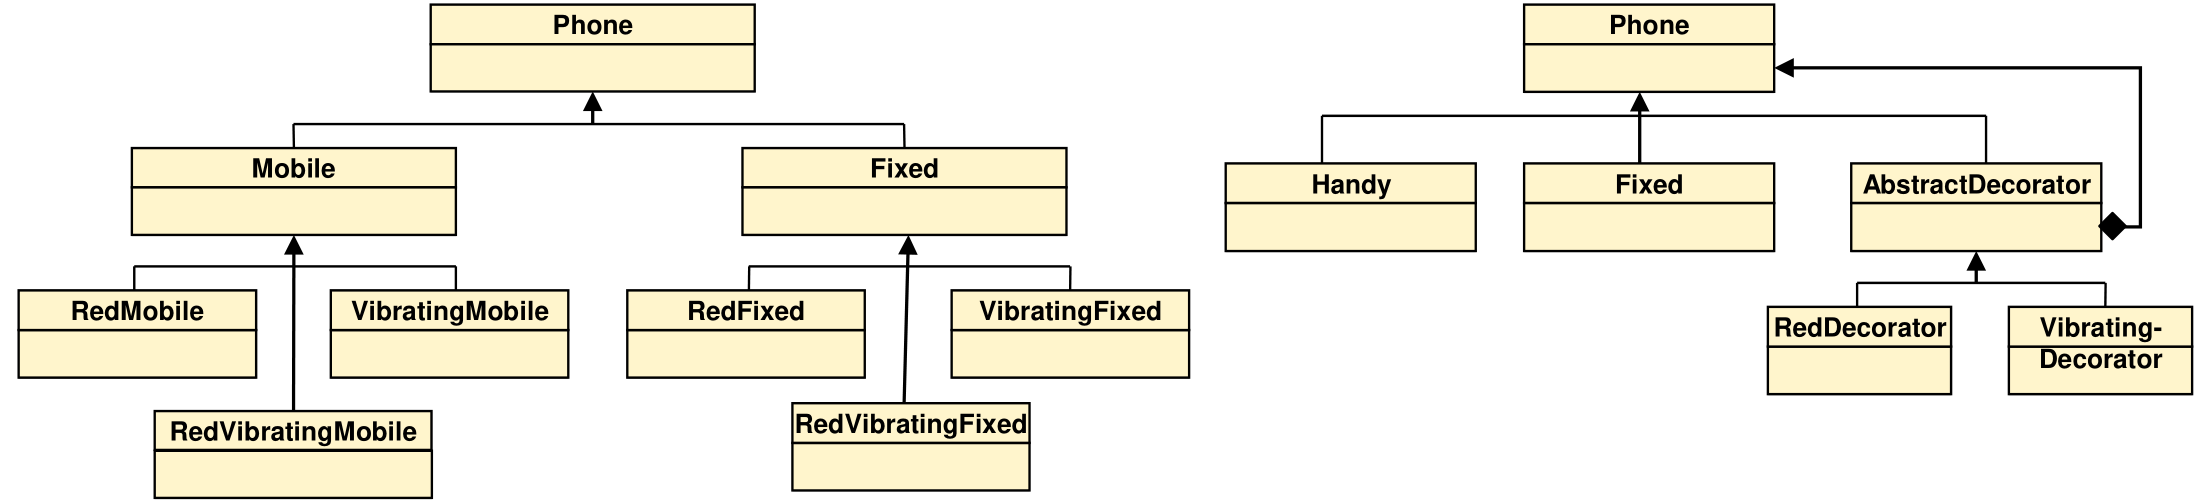
\includegraphics[width=1.0\textwidth]{figures/decoratorExplosion.png}
    \caption{Inheritance vs. Decoration}
    \vspace{-1em}
  \end{figure}
  \begin{align*}
    &n: \text{ number of properties}\\[-1\jot]
    &\text{\# of Subclasses with inheritance\&combination }&&2^n-1 \\[-1\jot]
    &\text{\# of additoinal Classes with decoration }&&n+1
  \end{align*}
\end{intentbox}
\begin{partbox}[Participants]
  \begin{itemizenosep}
    \item \imp{Basic building blocks}: is, or are they things that we want to
    decorate/add functionality to.
    \item \imp{Component Interface}: declares the shared methods of the basic
    building blocks that may be decorated by the decorator.\\
    The component interface is also implemented by the decorator.\\
    $\Rightarrow$ Leads to consistency between the decorator and the basic
    building blocks by declaring the methods that may be decorated.
    \item \imp{Decorator}: Is an \textit{optional}
    \begin{itemizenosep}
      \item abstract wrapper class that defines the shared methods and fields of
      the concrete decorators i.e.\ stores a reference to a basic building block
      or more commonly
        \item a wrapper class that
        \begin{itemize}
            \item stores a reference to the basic building block 
            \item simply calls the to be decorated methods of the reference to
          the building block
        \end{itemize}
    \end{itemizenosep}
      \item \imp{Client}: creates decorated classed by handing/decorating basic
      building blocks by decorators.
  \end{itemizenosep}
\end{partbox}
\begin{notebox}[Note]\nospacing
  A concrete Decorator class is useful if concreteDecorators do not decorate
  all methods that may possibly decorated!
\end{notebox}
\begin{codeboxNl}[Component e.g.\ Figure]{java}
  interface Component{
    public |\optc{type}| op1(|\optc{args}|);    // e.g. draw
    public |\optc{type}| op2(|\optc{args}|);    // e.g. setBounds
  }
\end{codeboxNl}
\begin{codeboxNl}[Concrete Component/Basic Building Block e.g.\ Rectangle]{java}
  class concreteCompA implements Component{
    public |\optc{type}| op1(|\optc{args}|){
        |\\optc{do something1}|
    };
    public |\optc{type}| op2(|\optc{args}|){
        |\optc{do something2}|
    }
  }
\end{codeboxNl}
\begin{codeboxNl}[Decorator]{java}
class Decorator implements Component{
  Component inner;
  public Decorator(Component inner){
    this.inner = inner;
  }
  // No decoration yet
  public |\optc{type}| op1(|\optc{args}|){
    inner.op1(|\optc{args}|);
  }

  public |\optc{type}| op2(|\optc{args}|){
    inner.op2(|\optc{args}|);
  }
}
\end{codeboxNl}
\begin{codeboxNl}[ConcreteDecorator e.g.\ ColorDecorator]{java}
class op1Decorator extends Decorator{
  @override
  public |\optc{type}| op1(|\optc{args}|){
    // Decorate before
    inner.op1(|\optc{args}|);
    // Decorate after
    addFunctionality(|\optc{args}|);
  }

  public |\optc{type}| addFunctionality(|\optc{args}|){
    // Do something
  }
}
\end{codeboxNl}
\begin{notebox}[Note]\nospacing
  \javainline{inner} may very well be another \javainline{concreteDecorator}
  and not a basic building block.
\end{notebox}
\begin{codeboxNl}[Client]{java}
  Oval ov = new Oval();
  RedColorDecorator redRec = new RedColorDecorator(ov);
\end{codeboxNl}
\begin{codeboxNl}[Client Example 2]{java}
  // MobilePhone implements Phone and has methods vibration and color
  MobilePhone m = new MobilePhone();
  RedColorDecorator redRec = new RedColorDecorator(ov);
  Phone redVibratingPhone =
          new RedColorDecorator(new VibrationDecorator(m));
\end{codeboxNl}
\begin{notebox}[Notes]\nospacing
  \begin{itemizenosep}
      \item May apply decorator before or after e.g.\
      may use decorator for some type safety checking
      \item 
  May also make sense to pass inner to setter method.
  \end{itemizenosep}
\end{notebox}
\subsubsection{Fields}
\label{subsubsec:Fields}
\begin{sectionbox}\nospacing
 Fields cannot be decorated explicitly \imp{but} if the basic building blocks
 use \javainline{getters} and \javainline{setters} then we may decorate them
 implicitly via those methods.
\end{sectionbox}
\begin{notebox}[Decorator vs State vs Strategy]\nospacing
  \begin{itemizenosep}
      \item A \tc{section}{Decorator} changes an object’s skin: that is it
    usually adds functionality (decorates) e.g.\ DrawTools may be decorators of
    the view.
      \item A \tc{section}{Strategy} changes an object’s guts: that is it is
      likely to change the internal strategy
      \item \tc{section}{State} changes an object’s guts: that is it is
      likely to changed its functionality completely 
  \end{itemizenosep}
\end{notebox}
\todo[inline]{Add type tests and problems (rest of slids)}
%%% Local Variables:
%%% mode: latex
%%% TeX-master: "../formulary"
%%% End:
